\section{Supplementary Figures}

\begin{figure}[H]
\centering
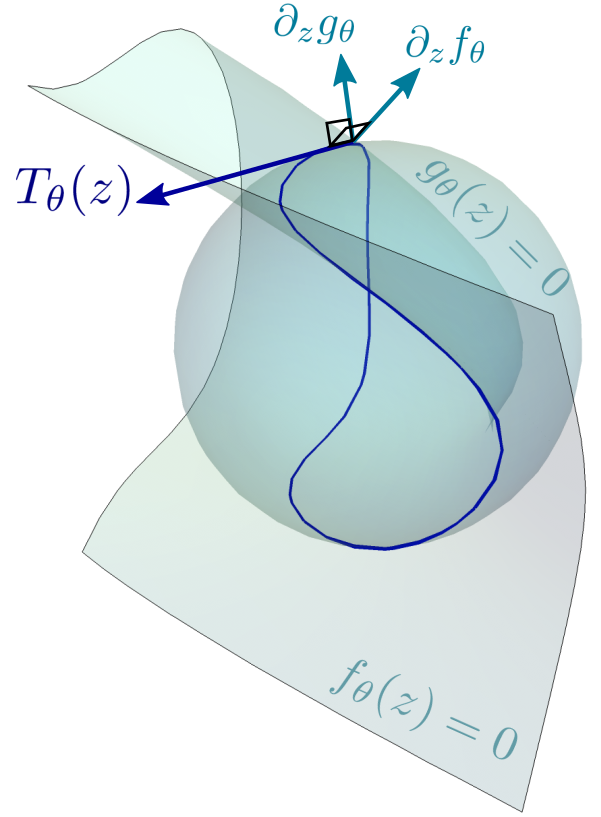
\includegraphics[width=5cm]{implicit-surfaces}
\caption{Two implicit surfaces $f_{\theta}(z)=0$ and $g_{\theta}(z)=0$ in $\mathbb{R}^3$ intersecting to form a space curve which is tangent to field $\tangent(z)$ and perpendicular to gradients $\partial_{z}f_{\theta}$ and $\partial_{z}g_{\theta}$}
\label{fig:implicit-surfaces}
\end{figure}

\section{Gradient of Space Curve}
\label{appendix:space-curve}

Suppose there exists a one dimensional space curve $\mathcal{C(\theta)}$ embedded in $z\in\Reals^{N+1}$ whos geometry changes depending on input parameters $\theta\in\Reals^M$. This curve could be open or closed and changes in $\theta$ could change the curve topology as well. Let the function $\gamma_{\theta}:\Reals\rightarrow\Reals^{N+1}$ be a parameterisation of the position vector along the curve within a fixed domain $s\in\mathcal{S}$. Note that the choice of parameterisation is arbitrary and our results should not depend on this choice. Furthermore, if we parametrise the curve $\mathcal{C}(\theta)$ with respect to a fixed domain $\mathcal{S}$ the dependence on $\theta$ is picked up by the parameterisation $\gamma_{\theta}(s)$. We can write a line integral of any scalar function $L_{\theta}:\Reals^{N+1}\rightarrow\Reals$ on the curve as
\begin{align}
    L(\theta):=
    \int_\mathcal{C(\theta)}\! L_{\theta}(z)\,\mathrm{d}z
    =\int_\mathcal{S}\! L_{\theta}(z)\left|\frac{d\gamma_{\theta}}{ds}\right|\mathrm{d}s_{\,\,z=\gamma_{\theta}(s)}
\end{align}
where $\left|\frac{d\gamma_{\theta}}{ds}\right|$ is the magnitude of tangent vectors to the space curve and we remind ourselves that the integrand is evaluated at $z=\gamma_{\theta}(s)$. We would like to track how this integral changes with respect to $\theta$. The total derivative with respect to $\theta$ can be propagated into the integrand \cite{Flanders1973DifferentiationSign} as long as we keep track of implicit dependencies
\begin{align}
    \frac{dL}{d\theta} &=\int_\mathcal{S}
    \left|\frac{d\gamma_{\theta}}{ds}\right|
    \left(
        \frac{\partial L}{\partial\theta}+
        \frac{\partial L}{\partial z}\cdot
        \frac{dz}{d\theta}
    \right)
    +L_{\theta}(z)\frac{d}{d\theta}\left|\frac{d\gamma_{\theta}}{ds}\right|
    \mathrm{d}s_{\,\,z=\gamma_{\theta}(s)}
    % \\&=\int_\mathcal{C(\theta)}
    %     \frac{\partial L}{\partial\theta}+
    %     \frac{\partial L}{\partial z}\cdot
    %     \frac{dz}{d\theta}
    % +L_{\theta}(z)\frac{d}{d\theta}\log\left|\frac{d\gamma_{\theta}}{ds}\right|
    % \mathrm{d}z
\end{align}
Here we applied the total derivative rule in the first term due to the implicit dependence of $z$ on $\theta$ through $z=\gamma_{\theta}(s)$. Applying the chain rule to the second term
\begin{align}
    \frac{d}{d\theta}\left|\frac{d\gamma_{\theta}}{ds}\right|=
    \left|\frac{d\gamma_{\theta}}{ds}\right|^{-1}
    \frac{d\gamma_{\theta}}{ds}\cdot\frac{d}{d\theta}
    \left(\frac{d\gamma_{\theta}}{ds}\right)
\end{align}
By choosing an $s$ that has no implicit $\theta$ dependence we can commute derivatives
\begin{align}
    \frac{d}{d\theta}\left(\frac{d\gamma_{\theta}}{ds}\right)
    = \frac{d}{ds}\left(\frac{d\gamma_{\theta}}{d\theta}\right)
    \quad\Rightarrow\quad
    \frac{d}{d\theta}\left|\frac{d\gamma_{\theta}}{ds}\right|=
    \left|\frac{d\gamma_{\theta}}{ds}\right|^{-1}
    \frac{d\gamma_{\theta}}{ds}\cdot\frac{d}{d s}
    \left(\frac{d\gamma_{\theta}}{d\theta}\right)
\end{align}
To proceed we note that the unit tangent vector can be written as an evaluation of a tangent field $\hat{T}_{\theta}(z)$ defined in the whole domain $z\in\Reals^{N+1}$ along the parametric curve $z=\gamma_{\theta}(s)$. The unit tangent field may disagree with the tangent given by $\frac{d\gamma_{\theta}}{ds}$ up to a sign
\begin{align}
    \left.\hat{\tangent}(z)\right|_{z=\gamma_{\theta}(s)}=
    \pm\left|\frac{d\gamma_{\theta}}{ds}\right|^{-1}\frac{d\gamma_{\theta}}{d s}
\end{align}
this leads to numerically verified result%\todo{perhaps not valid in general?}
\begin{align}
    \frac{d}{d\theta}\left|\frac{d\gamma_{\theta}}{ds}\right|=
    \left|\frac{d\gamma_{\theta}}{ds}\right|\left(
   \hat{\tangent}(z)\cdot\frac{\partial }{\partial z}\left(\frac{d\Gamma_{\theta}}{d \theta}\right)\cdot
   \hat{\tangent}(z)
    \right)_{z=\gamma_\theta(s)}
    \label{eq:divergence-term}
\end{align}

\section{Deformation of Implicit Surfaces}
\label{appendix:deformation}
It is possible to find the normal deformation of the implicit space curves due to changes in $\theta$. This can be done by taking the total derivative of the implicit equation defining the level set
\begin{align}
    \frac{d\rates(z)}{d\theta}=\frac{\partial F}{\partial\theta}+
    \frac{\partial F}{\partial z}\cdot\frac{d z}{d \theta}
\end{align}

We can rearrange for $\frac{d z}{d \theta}$ using the Moore-Penrose inverse of the rectangular Jacobian matrix $\frac{\partial F}{\partial z}$ which appeared in equation \eqref{eq:tangent-field}. Since the level set is defined by $\rates(z)=0$ the total derivative along the level set $d\rates(z)=0$ and we arrive at an expression for the deformation field \cite{Jos2011OnSurface}
\begin{align}
    \frac{d z}{d \theta} = - \frac{\partial F}{\partial z}^\top
    \left(\,
        \frac{\partial F}{\partial z}\,\frac{\partial F}{\partial z}^\top
    \right)^{-1}
    \frac{\partial F}{\partial\theta}
\end{align}
The tangential component of the deformation field is not uniquely determined because there is no unique way of parameterising a surface. This is the subject of many computer graphics papers \cite{Jos2011OnSurface,Tao2016Near-IsometricTracking,Fujisawa2013CalculationInvariance}. We are however not interested in the continuous propagation of a mesh - as is the subject of those papers. In fact we are looking for a deformation field that is orthogonal to the tangent vector $\hat{\tangent}(z) \cdot\frac{d z}{d\theta} =0$ for the space curve, and therefore letting the tangential component of the deformation equal zero is a valid choice and we can it instead of the parameterised deformation
% \todo{this is possibly quite shifty. Is this really valid?}
\begin{align}
    \frac{d \gamma_{\theta}}{d\theta} \rightarrow \frac{d z}{d\theta}
\end{align}
To summarise we now have the gradient of our line integral only in terms of the implicit function defining the integration region.
\begin{align}
    \frac{d L}{d\theta} =\int_{\rates(z)=0}
        \frac{\partial L}{\partial\theta}+
        \frac{\partial L}{\partial z}\cdot
        \varphi_{\theta}(z)
    +L_{\theta}(z)\,\,
    \hat{\tangent}(z)\cdot\frac{\partial \varphi}{\partial z}\cdot\hat{\tangent}(z)
    \,\mathrm{d}z\qquad\qquad\\
    \mathrm{where}\quad
    \hat{\tangent}(z):= \frac{\tangent(z)}{|\tangent(z)|}
    \qquad
    \tangent(z):=
    \left|\begin{matrix}
        \hat{z} \\
        \,\partial_{z}\rates\,
    \end{matrix}\right|
    \qquad
    \varphi_{\theta}(z) :=
- \frac{\partial F}{\partial z}^\top
    \left(\,
        \frac{\partial F}{\partial z}\,\frac{\partial F}{\partial z}^\top
    \right)^{-1}
    \frac{\partial F}{\partial\theta}
\end{align}
We have settled on choosing normal deformations which we will call $\varphi_\theta(z)$. The above result can be seen a the generalised Leibniz rule \cite{Flanders1973DifferentiationSign} for the case of line integration regions. The last integrand term can be seen as the divergence the vector field $\varphi_\theta(z)$ projected onto the one dimensional space curve.


\subsection{Bifurcation Curves as Tangent Fields}
\label{appendix:tangent-fields}

Let each component of the vector function $\rates$ in the model \eqref{eq:model} implicitly define a surface embedded in $\Reals^{N+1}$. Let's assume that the intersection of these $N$ surfaces exists and is not null or degenerate, then the steady states of \eqref{eq:model} must be a set of one dimensional space curves in $z\in\Reals^{N+1}$ defined by
\begin{align}
    \rates(z) = 0
\end{align}
An expression for the field $\tangent(z)$ tangent to the set of curves would allow us to take derivatives and integrals along the bifurcation curve. This is exactly what we need to do to evaluate our cost function \ref{eq:loss}. Fortunately the tangent field can be constructed by ensuring it is perpendicular to the gradient $\partial_z$ of each component of $\rates$ as illustrated by an example two component system in Figure \ref{fig:implicit-surfaces}. The tangent field $\tangent(z)$ can be constructed perpendicular to all gradient vectors using the properties of the determinant \cite{Goldman2005CurvatureSurfaces}
\begin{align}
    \tangent(z):=
    \label{eq:tangent-field}
    \left|\begin{matrix}
        \hat{z} \\
        \,\partial_{z}\rates\,
    \end{matrix}\right|
    \qquad\tangent : \Reals^{N+1}\rightarrow\Reals^{N+1}\\
    =\sum_{i=1}^{N+1}\hat{z}_{i}(-1)^{i+1} \left|\frac{\partial \rates}{\partial(z\setminus z_{i}) }\right|
\end{align}
where $\hat{z}$ is a collection of unit basis vectors in the $\Reals^{N+1}$ space and $\partial_{z}\rates$ is an $N\times(N+1)$ rectangular Jacobian matrix of partial derivatives and $z\setminus z_{i}$ denotes the $N$ dimensional vector $z$ with component $z_{i}$ removed. This construction ensures perpendicularity to any gradients of $\rates$
\begin{align}
    \tangent(z)\cdot\partial_z f_{\theta} =
    \left|\begin{matrix}
        \partial_z f_{\theta} \\
        \,\partial_{z}\rates\,
    \end{matrix}\right|
    \quad =0 \quad\forall f_{\theta}\in \rates
\end{align}
since the determinant of any matrix with two identical rows or columns is zero. Note that the tangent field $\tangent(z)$ is actually defined for all values of $z$ where adjacent field lines trace out other level sets where $\rates(z)\neq0$. Furthermore deformations with respect to $\theta$ are always orthogonal to the tangent
\begin{align} % \todo{numerically true. analytic proof?}
    \tangent(z)\cdot\frac{d\tangent}{d\theta}=0
\end{align}
\begin{figure}
\centering
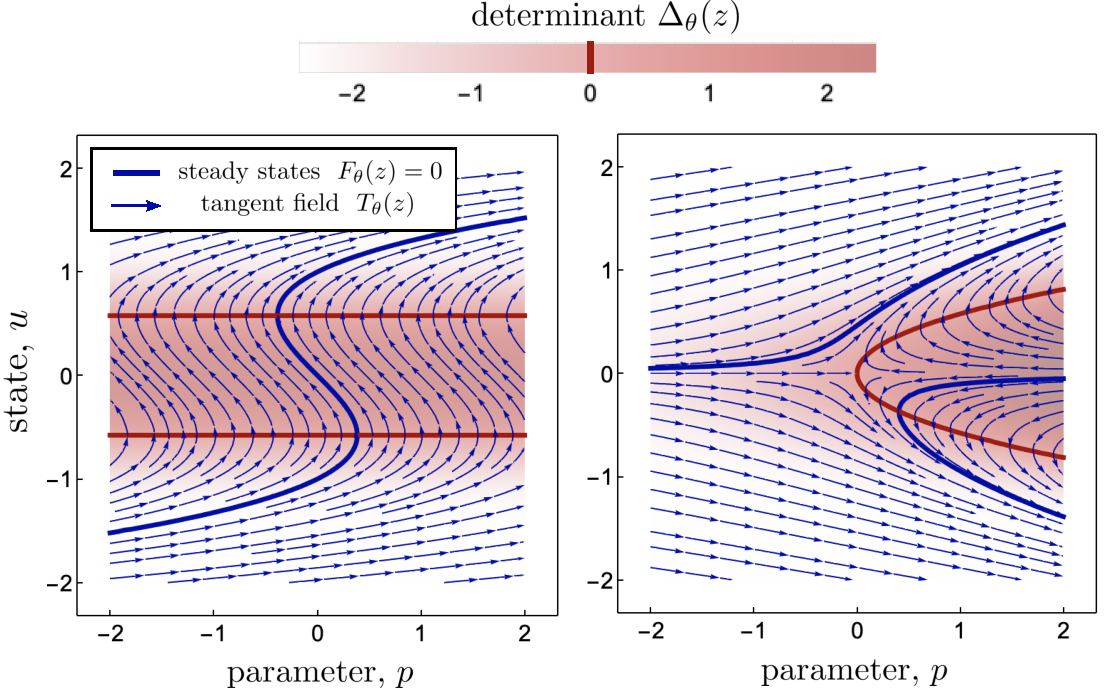
\includegraphics[width=13cm]{determinant-field}
\caption{Left/Right : Determinant $\Det$ and tangent field $\tangent(z)$ for the saddle-node/pitchfork models for some set values of $\theta$ revealing that $\Det=0$ defines bifurcations}
\label{fig:determinant-field}
\end{figure}
Figure \ref{fig:determinant-field} shows how the bifurcation curve defined by $\rates(z)=0$ picks out one of many level sets or traces in tangent field $\tangent(z)$ for the saddle and pitchfork. The tangent field $\tangent(z)$ can always be analytically evaluated by taking the determinant in \eqref{eq:tangent-field}. We will proceed with calculations on $\tangent(z)$ in the whole space $z$ and pick out a single trace by solving $\rates(z)=0$ later. For our two models
\begin{align}
    \underset{\mathrm{saddle-node\,\,model}}{
    \tangent(z)=\hat{u}-(\,3\theta_2 u^2+\theta_1\,)\,\hat{p}}
    \qquad\qquad
    \underset{\mathrm{pitchfork\,\,model}}{
    \tangent(z)=u\hat{u}-(\,3\theta_2 u^2+p\,)\,\hat{p}}
    \label{eq:tangent-field-examples}
\end{align}
Figure \ref{fig:determinant-field} reveals that $\Det=0$ is also a level set and that the intersection with level set $\rates(z)=0$ defines the bifurcations at specific parameter $\theta$. In this particular setting we can see that the tangent field $\tangent(z)$ only folds when $\Det=0$. Plotting the value of the determinant along $\rates(z)=0$ from Figure \ref{fig:determinant-field} would give rise to Figures \ref{fig:minimal-models}. The directional derivative of the determinant $\Det$ along the tangent field $\tangent(z)$ is defined as
\begin{align}
    \frac{d}{ds}\Det := \hat{\tangent}(z) \cdot \frac{\partial}{\partial z}\Det 
\end{align}
where $\hat{\tangent}(z)$ is the unit tangent field. 


\section{Bifurcation Measure}
\label{appendix:measure}


% \section{Simplification of two-state model}

% Consider the general two-state model:
% \begin{equation}
%     \dfrac{dv_i}{dt} = \dfrac{a_i + b_i (K_i v_j)^2}{1 + (K_i v_j)^2} - \mu_i v_i
% \end{equation}

% Without loss of generality, we can rescale $v_i = U_i u_i$. Then,
% \begin{equation}
%     \dfrac{U_idu_i}{dt} = \dfrac{a_i + b_i (K_i U_j u_j)^2}{1 + (K_i U_j u_j)^2} - \mu_i U_i u_i
% \end{equation}

% Dividing through by $U_i$, we obtain
% \begin{equation}
%     \dfrac{du_i}{dt} = \dfrac{\frac{a_i}{U_i} + \frac{b_i}{U_i} (K_i U_j u_j)^2}{1 + (K_i U_j u_j)^2} - \mu_i u_i
% \end{equation}

% By choosing $U_i = b_i$, the model reduces to:
% \begin{equation}
%     \dfrac{du_1}{dt} = \dfrac{\hat{a}_1 + (p u_2)^2}{1 + (p u_2)^2} - \mu_1 u_1, \quad
%     \dfrac{du_2}{dt} = \dfrac{\hat{a}_2 + (k u_1)^2}{1 + (k u_1)^2} - \mu_2 u_2
% \end{equation}
% where $p = \frac{K_1}{\sqrt{b_1}}$ and $k = \frac{K_2}{\sqrt{b_2}}$.